\documentclass[11pt]{article}
\usepackage[noadjust]{cite}
\usepackage{filecontents}

\usepackage[utf8]{inputenc}
\usepackage{authblk}
\usepackage{indentfirst}
\usepackage{tabularx}
\usepackage{makecell} % more specific table formatting
\newcommand{\bhline}{\Xhline{2\arrayrulewidth}}
\usepackage[margin=1.2in]{geometry} % changes all margins to 0.5 in
\usepackage{verbatim}
\usepackage{url}
\usepackage[bookmarks=true, colorlinks=true, linkcolor=blue!50!red, citecolor=blue,
pdfencoding=unicode]{hyperref}
\usepackage[round]{natbib}
\usepackage{subfloat}
\usepackage{caption}
\usepackage{subcaption}
\usepackage{graphicx} % include images
\graphicspath{{./images/}} % image paths
%\usepackage{subfig}
\usepackage{floatrow} % put an image and a table in the same row
\newfloatcommand{capbtabbox}{table}[][\FBwidth]
\bibliographystyle{unsrtnat}

\usepackage{mathtools} % math
\usepackage{amsthm}
\usepackage{amssymb}
\usepackage{fixltx2e} % wiring diagram imports
\usepackage[T1]{fontenc}
\usepackage{newpxtext}
\usepackage[varg,bigdelims]{newpxmath}
\usepackage[cal=euler,scr=rsfso]{mathalfa}
\usepackage{bm}
\usepackage{inputenc}
\usepackage{microtype}
\usepackage[usenames,dvipsnames]{xcolor}
\usepackage{paralist}
\usepackage{booktabs}
\usepackage{tikz}
\usepackage{makecell}
\usepackage{pgfplots}
\pgfplotsset{compat=1.11} % just for pgfplot
\usepackage{todonotes}
\usepackage[capitalize]{cleveref}


\usetikzlibrary{
	cd,
	decorations.markings,
	positioning,
	arrows.meta,
	shapes,
	calc,
	fit,
	quotes}


\newcommand{\tn}{\textnormal}
\newcommand{\inp}[1]{#1^{\tn{in}}}
\newcommand{\outp}[1]{#1^{\tn{out}}}
\newcommand{\upd}[1]{#1^{\tn{upd}}}
\newcommand{\rdt}[1]{#1^{\tn{rdt}}}

\usepackage{tabularx} % table

\addtolength{\topmargin}{-.25in}
\addtolength{\textheight}{.5in}

% ---- Wiring Diagram Preamble Starts

\tikzset{
	unoriented WD/.style={
		every to/.style={draw},
		shorten <=-\lsize, shorten >=-\lsize,
		label distance=-2pt,
		thick,
		node distance=\spacing,
		execute at begin picture={\tikzset{
			x=\spacing, y=\spacing}}
		},
	pack size/.store in=\psize,
	pack size = 8pt,
	spacing/.store in=\spacing,
	spacing = \psize,
	link size/.store in=\lsize,
	link size = 2pt,
	pack color/.store in=\pcolor,
	pack color = blue,
	pack inside color/.store in=\picolor,
	pack inside color=\pcolor!20,
	pack outside color/.store in=\pocolor,
	pack outside color=\pcolor!50!black,
	surround sep/.store in=\ssep,
	surround sep=\psize,
	link/.style={
		circle, 
		draw=black, 
		fill=black,
		inner sep=0pt, 
		minimum size=\lsize
	},
	pack/.style={
		circle, 
		draw = \pocolor, 
		fill = \picolor,
		inner sep = .25*\psize,
		minimum size = \psize
	},
	outer pack/.style={
		ellipse, 
		draw,
		inner sep=\ssep,
		color=\pocolor,
	},
	intermediate pack/.style={
		ellipse,
		dashed, 
		draw,
		inner sep=\ssep,
		color=\pocolor,
	},
}

% --- Wiring diagram preamble ends

\begin{document}

% \blindtext
%title and author details
\title{Using the Pixel Array Method to\\Numerically Analyze the Reaction-Diffusion Equation}
\author[1]{Cynthia T. Liu}
\author[2]{David I. Spivak}
\affil[1]{\small Massachusetts Institute of Technology, Department of Electrical Engineering and Computer Science}
\affil[2]{Massachusetts Institute of Technology, Department of Mathematics}
\date{}

\maketitle

%Abstract
\begin{abstract}
The Pixel Array (PA) Method, originally introduced by Spivak et. al., is a fast method for solving nonlinear or linear systems. One of its distinguishing features is that it presents all solutions within a bounding box, as a plot in a low number of ``exposed variables''. Here we develop a set-theoretic variant of the PA method, named the Pixel Array Solution-Set (PASS) method, that gives access to the other variable values. We use it to numerically find steady states for several partial differential equations, more specifically reaction diffusion equations. The robustness of the PASS method was tested on previously-solved reaction-diffusion equations, such as the heat and local Fisher equation, processed using finite differences. We go on to further analyze the equation
$\frac{\partial{n}}{\partial{t}} = \frac{1}{x^\gamma} \frac{\partial}{\partial{x}}\left(x^\gamma n^\delta \frac{\partial{n}}{\partial{x}} \right) + n^p$
for $p \ne \delta + 1$ from the work of Wilhelmsson and Jancel. We present patterns in the boundary conditions under which steady states can occur, thus giving new insight into the behavior of this equation.
\end{abstract}

\begin{center}
\line(1,0){350}
\end{center}

\section{Introduction}

Many physical systems are modeled using partial differential equations, which describe the relationship between changing variables in the system. The reaction diffusion equation is such an equation---or perhaps a family of such equations---used to model chemical reactions, population dynamics, plasma physics, and other physical phenomena. In one dimension, the general form of the reaction diffusion equation is:

\begin{equation}
    \label{Reaction-Diffusion Equation}
    u_t = D(x)u_{xx} + R(u) + f(x,t)
\end{equation}
where $D(x)$ is a general diffusion coefficient, $R(u)$ is the reaction, and $f(x,t)$ is a source or a sink.

Due to the ubiquity of \cref{Reaction-Diffusion Equation}, a large body of research has been developed to understand its behavior and solutions. General solutions several specific cases of reaction terms, including zero. For instance, a general solution to the Fisher equation $u_t = u_{xx} + \mu u(1-u)$, where $\mu$ is a constant, was derived by \citep{AnalyticFisher}.

However, a general solution to \cref{Reaction-Diffusion Equation}, or even just a general steady state analysis, has remained out of reach. Therefore, unsolved forms of the equation have been analyzed using numerical methods \citep{Numerical_RD_1, Numerical_RD_2, Numerical_RD_3}. These methods usually require initial and boundary conditions to be satisfied, and provide one numerical solution.

This is where the Pixel Array (PA) method \citep{Introduction_to_PA} becomes relevant. Unlike many other numerical methods, it provides all solutions to a system of equations within a bounding box and is often faster than quasi-Newton methods. Because partial differential equations can be converted to a system of equations using discrete approximation methods, the PA method can be applied to partial differential equations. However, as the PA method is quite new, we also undertake to test its accuracy in a few well-known cases.

To test and also use the PA method, we needed to adapt it so as to produce a matrix of full solution sets, rather than just boolean values indicating where solutions exist. We refer to this adapted method as the Pixel Array Solution-Set (PASS) method. The ``bounding box" in this case consists of a pair of ranges for boundary values, one on each side of the one-dimensional reaction-diffusion system; of course a higher-dimensional tensor of solution sets would be appropriate for a higher-dimensional system. Using the PASS method, we were able to quickly and efficiently search for steady states of reaction-diffusion equations, which do not appear to be well-understood.

The plan of the paper is as follows. In \cref{sec:methods} we provide a brief review of the finite differences method, as well as describe our modification of the PA method. In \cref{sec:verification} we use a combination of these methods to discretize the heat equation, the local Fisher equation, and what we will call the \textit{Wilhelmsson-Jancel} equation, and calculate numerical solutions. The first two of these, already being solved, allowed us to verify the accuracy of the PASS method.

Finally, we apply the method to variants of the Wilhelmsson-Jancel equation whose solutions and steady states appear to be unknown. The results of this work provides us insight into the behavior of the equation by suggesting a new hypothesis about equilibrium behavior, and by showing a pattern in the boundary values for which steady states might exist.

\section{Methods}\label{sec:methods}

The methods we use to numerically solve for steady states are described below. We first briefly illustrate our discretization method, finite differences. Then we describe the difference between the Pixel Array method of \citep{Introduction_to_PA} and the Pixel Array Solution-Set (PASS) method developed here. Finally, we demonstrate how using PASS with discretized partial differential equations lets us generate steady states.

% \todo[inline]{Introduce this section with a few lines.}
\subsection{Finite Differences}

\begin{comment}
Introduce set theoretic variant of pixel array method. Uses (blank) as addition, (blank) as multiplication, gives full solutions instead of merely indicating the presence of a solution. Use the homogeneous heat equation as an example.
\end{comment}

To apply the PASS method, we need to convert the reaction-diffusion equation \eqref{Reaction-Diffusion Equation} with $u_t = 0$ to an equation with no derivatives. This is done using finite differences, which uses secant lines to approximate derivatives. For instance,

\begin{equation}
    \label{FD second order}
    u_{xx} = \cfrac{1}{h^2} (u_{i+1} - 2u_i + u_{i-1})
\end{equation}

\noindent Where $h$ is the length of a discrete spatial interval in $x$, and $u_i$ corresponds to the discrete solution in the spatial interval $i$.\footnote{Note that in this example, we have a linear equation. This is because finite differences gives linear equations, but depending on the reaction-diffusion equation, the discretized form of that equation might not be linear.} When applied to the reaction-diffusion equation \eqref{Reaction-Diffusion Equation}---given that we are interested in steady states---this becomes:

\begin{equation}
    \label{discrete RD}
    0 = \cfrac{D}{h^2} (u_{i+1} - 2u_i + u_{i-1}) + R(u_i) + \hat{f}(x_i)
\end{equation}
Note that $f(x,t)$ in \cref{Reaction-Diffusion Equation} was changed to $\hat{f}(x_i)$, where $\hat{f}$ is a time-independent version of $f(x,t)$. This is because steady states are by definition independent of time, and thus we only care about the time-independent parts of the source or sink. 

Equations like \eqref{discrete RD} will be called \textit{discrete steady state conditions}. We will be solving systems of that equation for all i with the PASS method. If the discrete steady state condition is satisfied for all $u_i$, then the $u_i$ together in order form a numerical steady state.

\subsection{PASS: Modifying the Pixel Array method to pass along solution sets}\label{sec:PASS}

Each equation in the discretized system corresponds to an array in both the Pixel Array (PA) and PASS method. In \citep{Introduction_to_PA}, the PA method is executed with boolean k-dimensional matrices or tensors, each of which represents one equation (or inequality). Each of the $k$ dimensions in a given tensor specifies one variable of the corresponding equation, and each row or column in that dimension represents an interval of values the variable can assume. For each possible combination of $k$ variable values, the corresponding entry in the matrix is ``True" (1) if the equation is satisfied somewhere in that range of values and ``False" (0) otherwise. To represent this, we present Figure \cref{sample_function}, which is a function graph, and figure (\cref{sample_pixel_array}) as its corresponding pixel array with vertical dimension y and horizontal dimension x. Observe that the pixel array is upside down, to match conventions described in \citep{Introduction_to_PA}.

\todo[inline]{The writing on the graph is rotated by 90 degrees. Can you fix that by plotting the function in y,x coordinates, rather than rotating an x,y plot?}
\begin{figure}[h]
\begin{subfigure}{.4\textwidth}
  \centering
  \captionsetup{width=0.8\textwidth}
  \includegraphics[angle=-90,width=.7\linewidth]{"y equals x2".png}
  \caption{An example plot of a function, oriented so its axes match that of a matrix\\\vspace{.6in}}
  \label{sample_function}
\end{subfigure}%
\begin{subfigure}{.4\textwidth}
  \centering
  \captionsetup{width=0.84\textwidth}
  \includegraphics[width=.84\linewidth]{"pixel array".png}
  \caption{A low-resolution pixel array corresponding to the function plot. When the equation is satisfied at a vertex, we ``round up" in y. That means pixels adjacent to the vertex with y larger than y at the vertex are 1; the other adjacwnt vertices are 0.}
  \label{sample_pixel_array}
\end{subfigure}%
\caption{An example plot with its corresponding pixel array}
\label{plot_and_pa}
\end{figure}
% \todo{What does the second caption mean, ``round up in $y$''?}

In Figure (\ref{plot_and_pa}), each of the cells in Figure (\ref{sample_function}) corresponds to a pixel in Figure (\ref{sample_pixel_array}). For instance, the function $y=x^2$ goes through the cell with $x \in [-2,-1]$, $y \in [2,3]$, and therefore its associated pixel, the third pixel in the second row, has the value 1.

It is useful to set up a naming convention which relates the tensor entries and the cubes they correspond to. We thus refer to an entry by the value exactly at the center of its range; e.g. in the above example the pixel would be known as $(-1.5, 2.5)$. When we wish to refer to all of an entry's possible values as opposed to just the center value, we refer to it as a \textit{subcube}. We say that the \textit{bin-size}---meaning the width of each variable---for this pixel is $(1,1)$. For simplicity, we will assume that the bin sizes of all variables are equal, for every system we discuss.

Suppose each equation in the system has been plotted as a tensor, as above. To solve the simultaneous system of equations, these tensors are multiplied together by contracting various edges. The resulting tensor will then indicate all combinations of the remaining variables for which there exists a solution to the system.

What differentiates the PASS method is that we are interested in finding numerical steady states, not just determining their existence. Thus, the boolean definition of a pixel array is too limited. This is resolved by introducing a new data type, the \textit{solutionSet}. Each entry of our modified pixel array is of this data type. A solutionSet is a finite set of tuples of any finite length. In our work, the lengths of each tuple in a given solutionSet turn out to be the same, e.g.\  $\{(0,1,2), (1,1,1), (2,1,0)\}$, because they will represent the set of solutions---in certain selected variables---to some system of equations.

To get some intuition for the solutionSet data type, consider the homogeneous heat equation:

\begin{equation}
    \label{general homogeneous heat}
    u_t - D(x)u_{xx} = 0
\end{equation}

\noindent With $u_t = 0$ and $D(x) \equiv 1$, the equation becomes

\begin{equation}
    \label{homogeneous heat}
    u_{xx} = 0,
\end{equation}

\noindent otherwise known as the one-dimensional Laplace equation. After being processed by finite differences and multiplying both sides by $h^2 \ne 0$ we get: 

\begin{equation}
    \label{discrete heat}
    u_{i+1} - 2u_i + u_{i-1} = 0
\end{equation}

\noindent The corresponding tensor has three dimensions, corresponding to the variables $u_{i+1}$, $u_i$, and $u_{i-1}$ in \cref{discrete RD}. Each tensor entry corresponds to a subcube; let $(x,y,z)$ denote the center point of that subcube in space. The value in that entry will be the corresponding solution-set for the equation \cref{discrete heat}. That is, the value will be the empty set $\{\}$ if the subcube centered at $(x,y,z)$ does not contain a solution, and it will be the one-element set $\{(x,y,z)$\} if that subcube contains a solution.

Tensor multiplication involves multiplication and addition. For boolean values, multiplication is as usual, e.g.\ $1*0=0$, and addition is almost as usual, the exception being that $1+1=1$; this is the usual \emph{Boolean semiring}, which is used in the PA method. For the PASS method, we need to define multiplication and addition of the solutionSet data type. This data type will store the solutions to the local discrete steady state condition.

The multiplication of solutionSets is defined to be the Cartesian product of the tuples, and addition is defined to be set union. So if two theoretical solutionSets, \{(1),(2),(3)\} and \{(3,4)\} were multiplied, the resultant tuple would be \{(1,3),(2,3),(3,3),(1,4),(2,4),(3,4)\}. If they were added, we would get \{(1),(2),(3),(4)\}. This defines a commutative semiring, whose additive unit is the empty set $\{\}$ and whose multiplicative unit is $\{()\}$. Thus for example, when a solutionSet is multiplied by $\{\}$, the result is zero. When a solutionSet is added to $\{\}$ or multiplied by $\{()\}$, the solutionSet remains the same.

With this definition of multiplication, the generalized matrix multiplication algorithm remains the same as it was in \citep{Introduction_to_PA}.

\subsection{Producing Solutions}

We will now demonstrate how the above definition of the solutionSet data type allows us to compute numerical steady states to the reaction diffusion equation. Specifically, we will show how the numerical steady states are stored within solutionSets, and expanded as more multiplications are performed. 

We show this by example. Consider the heat equation \eqref{homogeneous heat} and its discrete version \eqref{discrete heat}. As discussed in \cref{sec:PASS}, all entries in the pixel array with dimensions $u_{i+1}$, $u_i$, and $u_{i-1}$ contain the single solution ${(u_i)}$ if $u_i$ satisfies \cref{discrete heat}. This is true for all partitions $i$.

With all the matrices defined, we will multiply them using the general matrix multiplication algorithm described in \cref{sec:PASS}, but to do so we must determine which variables are exposed. We resolve this by introducing the \textit{Wiring Diagram} (WD) for this system; see \cref{WD_heat}. As described in \citep{Introduction_to_PA}, the WD lets us connect matrices by their variables and lets us decide which variables we want to be exposed when we have finished multiplying.

\begin{figure*}
\caption{Wiring diagram for the discrete heat equation with n = 7 partitions. The boundary conditions in this instance are cells 1 and 5, but the product is evaluated as if 0 and 6 were boundaries to help prevent discontinuities at the true boundary.}
\label{WD_heat}
\begin{center}
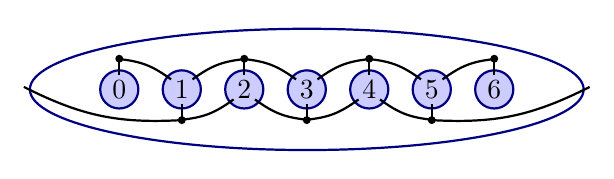
\begin{tikzpicture}[unoriented WD, surround sep= 3pt, every to/.style={draw, bend right=15pt}]
	\node[pack]                 (n0) {0};
	\node[pack, right=1 of n0]  (n1) {1};
	\node[pack, right=1 of n1]  (n2) {2};
	\node[pack, right=1 of n2]  (n3) {3};
	\node[pack, right=1 of n3]  (n4) {4};
	\node[pack, right=1 of n4]  (n5) {5};
	\node[pack, right=1 of n5]  (n6) {6};
	\node[link, above=.3 of n0] (l0) {};
	\node[link, above=.3 of n2] (l2) {};
	\node[link, above=.3 of n4] (l4) {};
	\node[link, above=.3 of n6] (l6) {};
	\node[link, below=.3 of n1] (l1) {};
	\node[link, below=.3 of n3] (l3) {};
	\node[link, below=.3 of n5] (l5) {};
	\node[outer pack, fit=(n0.center) (l2) (l3) (n6.center)] (outer) {};
%
	\draw (n0.north) -- (l0);
	\draw (n2.north) -- (l2);
	\draw (n4.north) -- (l4);
	\draw (n6.north) -- (l6);
	\draw (n1.south) -- (l1);
	\draw (n3.south) -- (l3);
	\draw (n5.south) -- (l5);
	\draw (n1) to (l0);
	\draw (n2) to (l3);
	\draw (n3) to (l2);
	\draw (n4) to (l5);
	\draw (n5) to (l4);
	\draw (l1) to (n2);
	\draw (l2) to (n1);
	\draw (l3) to (n4);
	\draw (l4) to (n3);
	\draw (l6) to (n5);
%
	\draw (outer.west) to (l1);
	\draw (l5) to (outer.east);
\end{tikzpicture}
\end{center}
\end{figure*}

In \cref{WD_heat}, the black dots (and the lines connecting them to circles) are called \textit{links}, while the circles are called \textit{cells} (in \citep{Introduction_to_PA} they were called \textit{packs}). Each cell represent one equation, its ports represent the variables of that equation, and the links represent the dependencies between variables. For example, because the equation for $u_i$ in \cref{discrete heat} depends on $u_{i+1}$ and $u_{i-1}$, there are links connecting the cells representing $u_{i+1}$, $u_{i-1}$, and $u_i$.

The last thing to explain about \cref{WD_heat} is the fact that we have both \emph{hidden boundaries}, cells 0 and 6, and the \emph{exposed boundaries}, cells 1 and 5. The boundary conditions found in the typical heat equation reference these exposed boundaries, and at first we did not include hidden boundaries. However, we found that in this case an anomaly can arise due to the spacial discretization in equations with a left-right asymmetry. For example, this problem does not arise for the heat equation or the Fischer equation \cref{discrete heat,discrete Fisher}, but it does arise for the Wilhelmsson-Jancel equation \cref{discrete WJ}. By adding the hidden boundaries, the anomaly vanishes.

\cref{WD_oneproduct} represents a multiplication of two 3-dimensional tensors $M_1$ and $M_2$, the result of which is a 4-dimensional tensor. (The dimension of a tensor is indicated in the diagram by its number of ports.) It is given by contracting along the links connecting $M_1$ and $M_2$, which represent shared dimensions. Performing multiple such tensor multiplications, one obtains the tensor multiplication indicated by \cref{WD_heat}.

% I don't know how to label the links

\begin{figure*}
\caption{Wiring diagram for a single product with 3 exposed variables and 4 total variables}
\label{WD_oneproduct}
\begin{center}
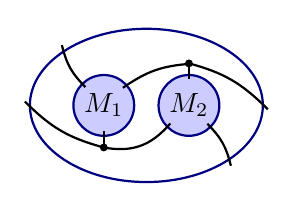
\begin{tikzpicture}[unoriented WD, surround sep= 3pt]
	\node[pack] (n1) {$M_1$};
	\node[pack, right=1 of n1] (n2) {$M_2$};
	\node[link, above=.3 of n2] (l2) {};
	\node[link, below=.3 of n1] (l1) {};
	\node[outer pack, fit={(n1) (n2) (l1) (l2)}] (outer) {};
	\draw (n1.south) -- (l1);
	\draw (n2.north) -- (l2);
	\draw (n1.north west) to[bend left=15pt] (outer.north west);
	\draw (n2.south east) to[bend left=15pt] (outer.south east);
	\draw (l1) to[bend right] (n2.south west);
	\draw (l2) to[bend right=15pt] (n1);
	\draw (l1) to[bend left=15pt] (outer.west);
	\draw (l2) to[bend left=15pt] (outer.east);
\end{tikzpicture}
\end{center}
\end{figure*}

Now that we know how to multiply matrices and determine exposed variables and boundary conditions, we use this knowledge to compute the value of a general solutionSet.  By the definition of solutionSet multiplication defined in Section 2.2, if the entry $\{(u_1)\}$ is multiplied by the entry $\{(u_2)\}$, the resulting solutionSet is $\{(u_1, u_2)\}$. Recall from \cref{sec:PASS} that the entry $\{(u_1)\}$ would only occur if \cref{discrete heat} were satisfied for that particular value. The same can be said for the entry $\{u_2\}$. Therefore, the product $\{(u_1, u_2)\}$ would only be produced if their values satisfied in \cref{discrete heat} for \textit{both} $i = 1$ and $i = 2$. This means that the final value within the solutionSet is a numerical steady states, because each local numerical solution fulfills the discrete steady state condition.

Thus, by multiplying all the matrices together, we calculate solutionSets of numerical steady states. Each element within a single solutionSet satisfies the discrete steady state condition locally. Furthermore, with the PASS method, we can calculate steady states for all possible pairs of left and right boundary values at once, in some sense parallelizing that computation.

\section{Verification}\label{sec:verification}

We will verify the accuracy of PASS by analyzing three reaction-diffusion equations. The first has no reaction term and a constant diffusion coefficient. The second has a nonconstant reaction term and constant diffusion coefficient. The last has both a nonconstant diffusion coefficient and nontrivial reaction term.

\subsection{Homogeneous Heat Equation}

We first consider the homogeneous heat equation as described by \cref{homogeneous heat}, whose discrete steady state condition is \cref{discrete heat}. It is well known that steady states to the homogeneous heat equation are linear between the two boundary conditions, and this fact can also be verified by directly solving the equation.

First, we will prove, for any number $n$ of cells, that the numerical solution converges to the true solution as the number of bins for a fixed range goes to infinity. This is equivalent to the bin size $b$ going to 0. We assume that all variables share the same number of bins and same possible values, due to the symmetry of the system.

An entry is nonempty if \cref{discrete heat} is fulfilled at some point within or on the edges of the entry. We know an entry contains a solution if any two vertices of the subcube have different signs (including 0). To prevent overcounting, we can check a fewer number of vertices, as long as edge cases are considered. This is our plotting method, or method of determining whether there is a solution within a subcube.

The coordinates at any vertex are $\pm \frac{b}{2}$ away from the center coordinates. So the maximum divergence from 0 at the center that still permits at least 1 vertex to have a different sign than the others (in this case 0) is $2b$. But equation \cref{discrete heat} is just the discrete second derivative. So that means:

\begin{equation}
    \label{max_diverge}
    |u_{xx}| \le 2b
\end{equation}

\noindent With $|u_{xx}| = 2b$ being the most an approximate solution can differ from a true solution. This goes to 0 as b goes to 0, and so the approximate solution must approach the true, linear, solution as $b$ approaches 0.

Given \cref{max_diverge}, we calculate a functional bound of the modified $L_2$ norm of $f(x_i) = u'_i-u_i$, where $u'_i$ is the discrete numerical solution at the value $x_i$ and $u_i$ is the value of the true solution at $x_i$. The bound is:

\begin{equation}
\label{n norm}
L = 2b \left \lceil \cfrac{n}{2} \right \rceil^{5/2}
\end{equation}

\noindent Which also goes to 0 as $b$ goes to 0. 

We run the program%
\footnote{The reader can find the program at \url{https://github.com/cynliu98/Pixel\_Array\_Python}, called \textit{general\_mat\_mult\_4.py}, in the archives folder.}
for a few combinations of $(b,n)$ to verify the bound in \eqref{n norm}. We checked the signs of the discrete steady state condition at four vertices per subcube. The program used a partition of $n=8$ parts and a temperature mesh of $b = .05$, giving 41 bins for each cell. The boundaries [1.9,0.55] gave a total of 11 steady states, some of which are shown in \cref{heats}. The largest modified $L_2$ norm among these solutions was . Thus, all modified norms are smaller than the bound determined by equation \cref{n norm}. The bound also holds for the steady states given by other pairs of boundaries. The runtime under these conditions was about 270 seconds in Python 3.

Therefore, the bound is accurate, and the numerical steady states calculated by PASS will converge to the correct states as $b \rightarrow 0$.

\begin{figure*}
\begin{center}
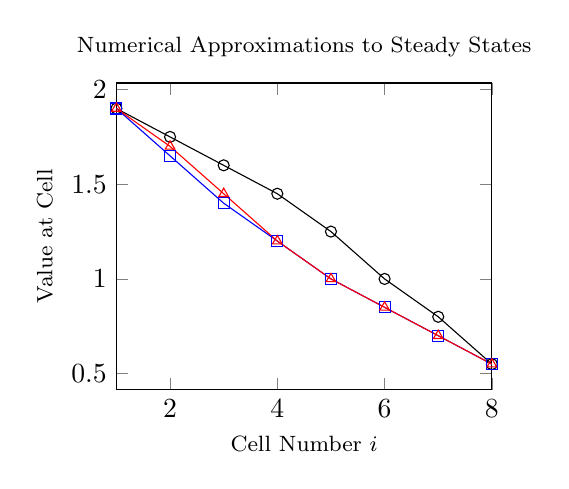
\begin{tikzpicture}
\begin{axis}[
title = \footnotesize Numerical Approximations to Steady States,
xlabel = \footnotesize Cell Number $i$,
ylabel = \footnotesize Value at Cell,
xmin = 1, xmax = 8,
width=2.5in
]
\addplot[black, mark=o] coordinates {
	(1, 1.9) 
	(2, 1.75)
	(3, 1.6)
	(4, 1.45)
	(5, 1.25)
	(6, 1)
	(7, .8)
	(8, .55)
};
\addplot[blue, mark=square] coordinates {
    (1, 1.9)
    (2, 1.65)
    (3, 1.4)
    (4, 1.2)
    (5, 1)
    (6, .85)
    (7, .7)
    (8, .55)
};
\addplot[red, mark=triangle] coordinates {
    (1, 1.9)
    (2, 1.7)
    (3, 1.45)
    (4, 1.2)
    (5, 1)
    (6, .85)
    (7, .7)
    (8, .55)
};
\end{axis}
\end{tikzpicture}
\caption{The numerical steady state approximations given for homogeneous heat equation with the boundaries [1.9,.55]}
\label{heats}
\end{center}
\end{figure*}

\subsection{Fisher-KPP Equation}

Now, we consider the classical Fisher-KPP equation \citep{Fisher}. In one dimension, the equation is:

\begin{equation}
    \label{Fisher}
    u_t = u_{xx} + \mu u (1-u)
\end{equation}

\noindent Where $\mu$ represents the intrinsic growth rate of a species \citep{Numerical_RD_1} when used in the field of population dynamics. Its corresponding steady state is:

\begin{equation}
    \label{discrete Fisher}
    0 = \cfrac{1}{h^2} (u_{i+1} - 2u_i + u_{i-1}) + \mu u_i (1-u_i)
\end{equation}

\noindent The only bounded steady states of this equation are $u \equiv 1$ and $u \equiv 0$ \citep{Fisher}, for all values of $\mu > 0$ and spatial interval size $h > 0$.

Our method of plotting the pixel arrays for this equation is different than plotting the array for the heat equation, because the Fisher equation is nonlinear. An outline of the method, which can also be used for all reaction diffusion equations, is:

\begin{enumerate}
    \item Let the discrete reaction diffusion expression be $f(u_{i+1}, u_i, u_{i-1})$, and calculate its value.
    \item  Round that expression to the nearest bin, and round 0 to the nearest bin\footnote{We can write possible bin values $b_j$ as $b_j = mj + c$ for $j \in \mathbb{Z}$, $j \in [0,r]$ where $r$ is the resolution. However, we can expand this definition and remove the last condition on $j$. We round off to the nearest of these expanded bin values}. If those rounded values are the same, then the corresponding entry in the Pixel Array is nonempty.
\end{enumerate}

This method obviously converges as the size of bins $b \rightarrow 0$, because $f(u_{i+1}, u_i, u_{i-1})$ and 0 must round to the same expanded bin and smaller $b$ restricts the range of values that could round to the same bin. This is true for any fixed spatial interval size $h$, including as $h \rightarrow 0$.

We run the program with 40 bins, $b = .051$ in the range $[0,2]$ and 10 cells, rounding up. We first test 3 values of $h$, $h = 1$, $h = .25$, and $h = .1$, all with $\mu = 1$. Because there are far significantly fewer steady states (just $u \equiv 1$ and $u \equiv 0$), we check for two things when verifying the PASS method. The method must give $u \equiv 1$ and $u \equiv 0$ if those are possible solutions, and preferably approximate solutions that are similar to those if those exact values are not possible. Furthermore, the must not give too many false positives. We present Tables 1(a) and 1(b) as well as some data to show that the PASS method fulfills these requirements

\begin{comment}
\footnote{Ok, does it?}.
\end{comment}

\begin{table}
\begin{center}

\begin{tabular}{ | c | c | }
\hline
$n$ & Number of Steady States \\
\bhline
4 & 37 \\
\hline
6 & 2 \\
\hline
8 & 2 \\ 
\hline
16 & 2 \\
\hline
32 & 2 \\
\hline
\end{tabular}
\hspace{.5in}
\begin{tabular}{ | c | c | }
\hline
$\mu$ & Number of Steady States \\
\bhline
.2 & 8 \\
\hline
.5 & 4 \\ 
\hline
2 & 1 \\ % Ok fam we have a problem. I think this is not ok
\hline
5 & 1 \\
\hline
\end{tabular}

\caption{Number of steady states in terms of $n$ and $\mu$.}
\label{Fisher Statistics}
\end{center}
\end{table}

The two steady states reported for $n \ge 6$ are $u_i \equiv .974$ and $u_i \equiv 0$ for all i. The program used .974 instead of 1 because 1 is not a possible bin, and $.974$ is the closest bin to 1. Both of these steady states were reported for $n = 4$, but it also included many more solutions because dividing the same space into coarser intervals (larger $h$, smaller $p$) allows for greater variation among steady states.

Then, for $n = 16$, we tested $\mu = .2$, $\mu = .5$, $\mu = 2$, and $\mu = 5$ ($\mu = 1$ had already been tested in \cref{Fisher Statistics}(a)). The results are in \cref{Fisher Statistics}(b). All of the additional steady states for $\mu = .2$ and $\mu = .5$ were also constant steady states . For $\mu = .2$ they were $u_i \equiv .051$, .103, .872, .923, .974, 1.026, and 1.077. For $\mu = .5$ $u_i \equiv .051$ and $1.026$ were the extra steady states. $u_i \equiv 1$ and $u_i \equiv 0$ were reported for all $\mu \le 1$. For $\mu \ge 2$, the approximation of $u_i \equiv 1$ was removed, while the solution $u_i \equiv 0$ remained. This is because 1 is not an allowed approximate solution value when $b = .051$ in the range [0,2], but 0 is. For $u_i \ne 1$ or $0$ and sufficiently large mu, the magnitude of the source term in \cref{discrete Fisher} is too large for the entire right hand side of the equation to round to 0. In other words, the false negative is the result of our discretization the solution space, and not of the PASS negative.

To confirm that discretization is indeed the issue, if $b = .05$ instead of $b = .051$, then the two solutions $u_i \equiv 0$ and $u_i \equiv 1$ always appear, regardless of $\mu$. This is because the expression \eqref{discrete Fisher} evaluates to exactly 0. Therefore, the PASS method identifies all true steady states, while it is not guaranteed to accept rough approximations to those steady states.

\subsection{Wilhelmsson-Jancel Equation}

Finally, we apply PASS to the following equation:

\begin{equation}
    \label{WJ}
    \cfrac{\partial{u}}{\partial{t}} = \cfrac{1}{x^\gamma} \cfrac{\partial}{\partial{x}} \left( x^\gamma au^\delta \cfrac{\partial{u}}{\partial{x}} \right) + cu^p
\end{equation}

Which was the subject of the paper ``Self-generation and nonlinear diffusion---an analytic approach" \citep{WJ}. As the equation is unnamed, we will refer to it as the ``Wilhelmsson-Jancel" equation, after the authors' names. By setting $D = au^\delta$ and performing two coordinate changes to eliminate constants, the authors simplify \cref{WJ} to:

\begin{equation}
  \label{Simplified WJ}
  \cfrac{\partial{u}}{\partial{t}} = \cfrac{1}{1+\delta} \cfrac{1}{x^\gamma} \cfrac{\partial}{\partial{x}}\left(x^\gamma \cfrac{\partial{u^{\delta + 1}}}{\partial{x}} \right) + u^p
\end{equation}

In \citep{WJ}, the authors derive an exact solution for $p = \delta + 1$, for 1 dimensional space or $\gamma = 0$. If one lets $t \rightarrow \infty$, one can see that the only bounded steady state is $u_i \equiv 0$ for all i.

The discrete steady state condition of this equation with $\gamma = 0$ is, calculated with forward differences is:

\begin{equation}
  \label{discrete WJ}
  0 = \cfrac{1}{h^2} \left[ u_{j}^\delta (u_{j+1} - u_{j}) - u_{j-1}^\delta (u_{j} - u_{j-1}) \right] + u_{j-1}^p
\end{equation}

With $h = .1$, we test three combinations of $(p, \delta)$ such that $p = \delta + 1$ and report the number of solutions in \cref{WJ Statistics}. All other settings remain the same.

\begin{table*}
\begin{center}
\label{WJ Statistics}
\begin{tabular}{ | c | c | }
\hline
$(p, \delta)$ & Number of Steady States \\
\hline
(2,1) & 78 \\
\hline
(3,2) & 88 \\ 
\hline
(1.5, .5) & 78 \\
\hline
\end{tabular}
\setcounter{table}{1}
\caption{$(p, \delta)$ vs. Number of numerical steady states given $h = .1$}
\end{center}
\end{table*}

If $u_i \equiv 0$ is theoretically the only steady state, it seems odd that there are so many reported steady states. However, these extraneous steady states are a result of discretization, not the PASS method. Furthermore, it is easy to eliminate false positives by making two observations: that steady states must be differentiable, and that the value of the right hand expression in \cref{discrete WJ} must tend to 0 as $b \rightarrow 0$. 

Most of the reported steady states, in the limit case of $n \rightarrow 0$, become a delta distribution. This distribution is not differentiable, and therefore these reported steady states must be false positives. The remaining extraneous steady states are constant at $u_i \equiv k$ for small k. This was permitted because the diffusion term (term dependent on $h$) in equation \cref{discrete WJ} is 0 for all constant solutions\footnote{This makes intuitive sense because there no net diffusion in a constant concentration system}, leaving only the requirement that $\text{round}(u_{j-1}^p) - \text{round}(0) < \frac{b}{2}$\footnote{where rounding is to the nearest extended bin}. Clearly, as $b \rightarrow 0$, $u_{j-1}$ and therefore $k$ must go to 0.

Thus, it is easy to eliminate extraneous solutions, and verify that $u_i \equiv 0$ is the only steady state to the Wilhelmsson-Jancel equation with $\gamma = 0$ and $p = \delta + 1$.

\section{Further analysis of Wilhelmsson-Jancel}

As mentioned previously, PASS, unlike other numerical methods, can find many steady states at once. Thus, the PASS method can quickly reveal patterns in the type of system boundaries that could produce an equilibrium state, and enables researchers to compare patterns among similar systems. We do this by plotting a binary matrix that indicates whether a solution was found for the corresponding set of boundaries\footnote{Note that such a binary matrix is identical to a pixel array as described by \citep{Introduction_to_PA}. In fact, we can achieve identical results by using the PA method as opposed to the PASS method}.

For instance, for the Wilhelmsson-Jancel equation with $(p, \delta) = (2,1)$, we can produce a plot of fulfilled boundaries (which we call a \textit{boundary plot}) as shown in \cref{21plot}. This figure, along with the analysis provided in section 3.3 that removes extraneous solutions that are cirlced in the figure, give results consistent with those given in \citep{WJ}. Thus, in this section we move on to cases that do not appear to have been analyzed previously.

\begin{figure}[h]
\begin{center}
\includegraphics[scale=.3]{images/"WJ 2-1".png}
\caption{Graph of fulfilled boundaries in the range [0,2] for $(p, \delta) = (2,1)$. The left boundary value is on the vertical axis, while the right boundary value is on the horizontal}
\label{21plot}
\end{center}
\end{figure}

We can compare plots and solutions for various combinations of $(p, \delta)$ to the plot and solutions for $(p, \delta) = (2,1)$. We focus on $p \ne \delta + 1$, a case mentioned in passing in \citep{WJ}. Through these comparisons we can establish hypotheses about which combinations of $(p, \delta)$ cause \cref{WJ} to have similar solutions and the same steady states as for $(p, \delta) = (2,1)$. Our analysis indicates that for $p > 1$, $\delta > 0$, the system's equilibrium behavior is very similar. It also suggests that systems whose $p$ and $\delta$ have different signs might have no equilibria at all, stable or unstable. 

We present boundary plots of the cases $(p, \delta) = (3,1), (4, 2), (1.5, 1), \text{and } (2,3)$ in \cref{large_positive_plot}. As one can see, the boundary plots are very similar to \cref{21plot}.

\begin{figure}[h]
\begin{subfigure}{.25\textwidth}
  \centering
  \includegraphics[width=.9\linewidth]{"WJ 31".png}
  \caption{$(p, \delta) = (3,2)$}
  \label{31plot}
\end{subfigure}%
\begin{subfigure}{.25\textwidth}
  \centering
  \includegraphics[width=.9\linewidth]{"WJ 42".png}
  \caption{$(p, \delta) = (4,2)$}
  \label{42plot}
\end{subfigure}%
\begin{subfigure}{.25\textwidth}
  \centering
  \includegraphics[width=.9\linewidth]{"WJ 1ah1".png}
  \caption{$(p, \delta) = (1.5,1)$}
  \label{1ah1plot}
\end{subfigure}%
\begin{subfigure}{.25\textwidth}
  \centering
  \includegraphics[width=.9\linewidth]{"WJ 23".png}
  \caption{$(p, \delta) = (2,3)$}
  \label{23plot}
\end{subfigure}
\caption{Boundary plots}
\label{large_positive_plot}
\end{figure}

All the circled areas in the plots are a result of discretization, not of PASS. This is because discretization removes the requirement for a solution to be differentiable. 

A glance over the steady states reveals that all of the reported steady states are similar to those reported for $(p, \delta) = (2,1)$. In each plot in \cref{large_positive_plot}, all reported steady states with $u_i = 0$ match those reported for $(p, \delta) = (2,1)$. Also in all plots, those steady states for boundary pairs along the main diagonal are constant steady states at the value of the boundary. As previously discussed, the diffusion term of constant solutions is 0, and thus we only need $\text{round}(u_{j-1}^p) - \text{round}(0) < \frac{b}{2}$. As $p$ increases, but $b$ stays constant, one can see that the number of possible $u_{j-1}$ increases, but $u_{j-1}$ remains less than 0. 

In the last plot, the reported steady states with $u_0 = .05$ are identical to those reported for $u_0 = 0$. Plugging the discrete solution values at the left boundary into \cref{discrete WJ}, we see that for sufficiently small values of $u_0$, the diffusion term is very small due to the relatively large value of $\delta$. At the left boundary, with $(u_2, u_1, u_0) = (0,0,k)$, and $(p, \delta) = (2,3)$, the steady state condition simplifies to $\text{round}(k^4 + k^2) - \text{round}(0) < \frac{b}{2}$. Again, as $b \rightarrow 0$, the largest of those sufficienty small values will go to 0. Thus, after eliminating extraneous solutions in a similar manner to that described in section 3.3, we hypothesize that for any $p > 1, \delta > 0$, $n \equiv 0$ is the only steady state of the Wilhelmsson-Jancel equation.

Because so many boundaries are tested at once, the results may also indicate that no steady states exist for certain parameters. For instance, we note that the explicit restrictions set on $p$ and $\delta$ if $p = \delta + 1$ in \citep{WJ} are not sufficiently restrictive. \citep{WJ} claim that their solution is accurate for all $p = \delta + 1$ if $p \ne 1$ and $\delta \ne 0$, whereas $n \equiv 0$ is not a steady state if $p$ or $\delta < 0$. This is easily verifiable using \cref{WJ}. 

However, the PASS method can suggest other hypotheses that are not as easily verified. For the following $(p, \delta)$, there are no steady states in either of the ranges $[0,2]$ and $[8,10]$, and we hypothesize that in these cases for $\gamma = 0$ \cref{WJ} has no equilibria for only positive solutions ($n \ge 0$): (0,1), (0, -2), (0, 3), (-1,1), (1, -2).

In all of these cases with no reported steady states, p and $\delta$ have different signs. This is true even when $p \ne \delta + 1$, and neither of their values is less than 0. Therefore, we may hypothesize that when p and $\delta$ have different signs (where 0 is also a different sign), the system has no equilibria. 

In conclusion, the PASS method suggests that the Wilhelmsson-Jancel equation has no nontrivial steady states for $p > 1$, $\delta > 0$, and that it has no equilibria at all for $p$ and $\delta$ with different signs.

\begin{comment}
\section{Analyzing the nonlocal Fisher equation}
Ask if this should be included for more variety, maybe legitimacy because relevant research is more recent? Thanks Stanford.
\end{comment}

\section{Conclusion}

The PASS method may be used to analyze reaction diffusion equations, by discretizing those equations and using PASS to numerically solve the resulting system. A rough estimate of many steady states can be achieved with the provided program in Python. However, a Julia (or other computational language) implementation can run much more powerful estimations extremely quickly. The PASS method may be extended to find steady states of other one-dimensional partial differential equations and two- or three-dimensional systems. This is done by adjusting the steady state condition, and pixel array creation algorithms based on the discretization and wiring diagram of the new equation.

The primary novel benefit of the PASS method is the parallelizing the computation of many steady states. By doing so, it can reveal patterns in the behavior of equilibria much more efficiently than other numerical methods. Furthermore, as demonstrated in section 4, results of PASS may be used to establish hypotheses about steady state behavior of a little-understood equation.

The PASS method has the same limitations as the original PA method, such as producing false positives, and the additional limitation of possible false negatives. Furthermore, discretization methods like finite difference eliminate derivatives from the equation entirely, and thus it is important to verify that the reported steady states are differentiable in the limit case of $n \rightarrow \infty$. However, any false positives due to this are caused by discretization, and not the PASS method. Similarly, false negatives, which are far rarer than false positives, are caused by discretization in the solution space, and not the PASS method.

\section{Acknolwedgments}

\begin{comment}

% Use ONLY if UROP advisor is not author

I would like to thank my UROP advisor, Dr. David Spivak, for his guidance, encouragement, and insight in helping me understand and conduct independent research into the pixel array method. I would also like to thank Professor Steven Johnson for the inspiration for this project.

\end{comment}

We thank our sponsors for the opportunity to do this research: CTL was sponsored by the MIT UROP program, and DIS was sponsored by AFOSR grants FA9550-14-1-0031 and FA9550-17-1-0058. We would also like to thank Professor Steven Johnson for suggesting this project to us.

\begin{comment}

\section{APPENDIX}

\subsection{Proof of Bounds for Heat Equation Approximation}

The modified $L_2$ norm we use in this proof is:

\begin{equation}
\label{L_2}
L_2 = \left(\sum_{i=1}^p (u'_i - u_i)^2\right)^{1/2}
\end{equation}

\cite{FD_convergence} defines it slightly differently, using the spatial grid size as a variable. However, we are varying the number of bins while keeping the number of cells constant. A constant coefficient does not change limit behavior, so we do not consider the size of the grid.

I will prove convergence for the closest numerical approximation to the worst case scenario describe by \cref{max_diverge}. The closest numerical approximation to the worst case scenario sets the value of \cref{discrete heat} at the center of each subcube to be $\pm 2b$. We will assume homogeneous trivial boundaries $u_0 = u_{p+1} = 0$, and then at the end I will briefly explain how to generalize to arbitrary boundaries.

Let the bin size, or difference between adjacent bins, be $b$. The worst case scenario values are as follows:

For p odd:
\begin{align}
\begin{split}
\label{p odd}
    u_1 &= 2\lceil \cfrac{p}{2} \rceil b \\ 
    u_2 &= 2 (\lceil \cfrac{p}{2} \rceil + \lceil \cfrac{p}{2} \rceil - 1) b \\ 
    \vdots \\
    u_{\lceil \frac{p}{2} \rceil} &= \sum_{j=1}^{\lceil \frac{p}{2} \rceil} 2jb \\
    u_{p + 1 - j} &= u_j
\end{split}
\end{align}

We can show that this is possible by observing how, in the theoretical case of $b = 1$, $u_{i-1} = 0$, $u_i = 4$, and $u_{i+1} = 6$ is possible. One of the vertices of this subcube has coordinates $(u_{i-1}, u_i, u_{i+1}) = (.5, 3.5, 6.5)$, which fulfills the discrete steady state condition. However, it is also implied that a larger deviation from local linearity would not be accepted by the program.

For p even, the values are similar but slightly altered:
\begin{align}
\begin{split}
\label{p even}
    u_1 &= 2\lceil \cfrac{p}{2} \rceil b \\ 
    u_2 &= 2 (\lceil \cfrac{p}{2} \rceil + \lceil \cfrac{p}{2} \rceil - 1) b \\ 
    \vdots \\
    u_{\lceil \frac{p}{2} \rceil} &= \sum_{j=1}^{\lceil \frac{p}{2} \rceil} 2jb \\
    u_{p + 1 - j} &= u_j
\end{split}
\end{align}

The $L_2$ norm is for p odd is then:

\begin{align}
\begin{split}
\label{p odd norm}
||u|| &= \left(\sum_{i=1}^p (u_i)^2\right)^{1/2} \\
&= 2b \left(\sum_{i=1}^{\lceil \frac{p}{2} \rceil} (\sum_{j=\lceil \frac{p}{2} \rceil + 1 - i}^{\lceil \frac{p}{2} \rceil} j)^2 \right)^{1/2} \\
&\le 2b \left(\sum_{i=1}^{\lceil \frac{p}{2} \rceil} (\sum_{j=\lceil \frac{p}{2} \rceil + 1 - i}^{\lceil \frac{p}{2} \rceil} \lceil \cfrac{p}{2} \rceil)^2 \right)^{1/2} \\
&\le 2b \left(\sum_{i=1}^{\lceil \frac{p}{2} \rceil} (\sum_{j=1}^{\lceil \frac{p}{2} \rceil} \lceil \cfrac{p}{2} \rceil)^2 \right)^{1/2} \\
&= 2b \left(\lceil \cfrac{p}{2} \rceil^5 \right)^{1/2}
\end{split}
\end{align}

Similarly $L_2$ norm for p even is:

\begin{equation}
\label{p even norm}
= 2b \left(\cfrac{p}{2} \right)^{5/2}
\end{equation}

And thus, for a fixed p, we see that the $L_2$ norm converges to 0 at a rate of $O(b)$, where the arbitrary sequence $\{b_n\}_{n=1}^\infty$ converges towards 0.\footnote{it does not matter in this case how the sequence converges to 0, only that it does.}

\end{comment}

\section{REFERENCES}

\bibliography{sources}

\end{document}
